% 05-Results.tex -- results exhibits, AAAI 2027 two-column layout.
%
% AAAI COMPLIANCE: uses only packages already loaded by the template
% (graphicx, booktabs, caption) -- no threeparttable, no added packages --
% and none of the commands aaai2027 forbids: no \setlength, \addtolength,
% \vspace, \vskip, \newpage, \pagebreak, \clearpage, \linespread,
% \baselinestretch or \tiny. Column padding is trimmed with @{} in the
% column spec rather than by resetting \tabcolsep. Wide exhibits use
% table*/figure*; table notes are plain footnotesize lines.
%
% Figure files: net_curves.pdf, islands_scaling.pdf.
\providecommand{\se}[1]{{\scriptsize$\pm$#1}}
% Fallbacks so this file compiles even if the preamble's \usepackage{booktabs}
% line is commented out (it ships commented in some template revisions).
% These are no-ops when booktabs is loaded.
\providecommand{\toprule}{\hline}
\providecommand{\midrule}{\hline}
\providecommand{\bottomrule}{\hline}

\section{Results}

\begin{table*}[t]
\centering
\small
\begin{tabular}{@{}lrrrr@{}}
\toprule
 & 2022 & 2023 & 2024 & 2022--24 \\
\midrule
ONE-NAS (60 isl., sleeves book)              & $+6.9$\se{0.7}  & $+13.7$\se{0.6} & $+7.0$\se{0.5}  & $+30.1$\se{0.9} \\
ONE-NAS (40 isl., sleeves book)              & $+6.1$\se{0.8}  & $+12.4$\se{0.7} & $+6.3$\se{0.5}  & $+27.5$\se{1.1} \\
ONE-NAS (20 isl., sleeves book)              & $+5.1$\se{0.5}  & $+13.3$\se{1.0} & $+6.3$\se{0.6}  & $+27.4$\se{1.1} \\
\midrule
ONE-NAS (40 isl., banded book)$^{a}$         & $+12.5$\se{1.2} & $+14.6$\se{1.3} & $+3.4$\se{0.9}  & $+33.9$\se{1.8} \\
ONE-NAS (40 isl., Algorithm 1 book)$^{b}$    & $+1.3$\se{1.6}  & $+12.8$\se{1.0} & $+10.8$\se{1.2} & $+25.0$\se{1.8} \\
\midrule
ONE-NAS single champion (60 isl.)$^{c}$      & ---             & ---             & ---             & $+1.0$ \\
ONE-NAS single champion (20 isl.)$^{c}$      & ---             & ---             & ---             & $+4.7$ \\
Online LSTM                                  & $+1.2$\se{1.3}  & $+4.5$\se{1.2}  & $+3.8$\se{0.7}  & $+11.3$\se{1.8} \\
Online GRU                                   & $+2.1$\se{1.0}  & $+3.1$\se{1.9}  & $+5.0$\se{0.8}  & $+11.7$\se{2.2} \\
Periodic LSTM (monthly retrain)              & $+1.4$\se{1.0}  & $+3.9$\se{0.8}  & $+6.9$\se{0.6}  & $+14.8$\se{1.0} \\
Online AR$^{d}$                              & $-14.6$         & $+4.8$          & $+7.9$          & $-3.3$ \\
\midrule
Buy \& hold$^{e}$                            & $-10.1$         & $+11.2$         & $+6.8$          & $+7.9$ \\
\bottomrule
\end{tabular}
\par\smallskip
{\footnotesize
$^{a}$Buy/hold-spread rule (enter rank $\le$10, exit past 35); sensitivity
row, not an adopted headline.
$^{b}$Conditional long--short book (rebalance only when all top-10
predictions are positive and all bottom-10 negative); on rank-normal
predictions the gate fires daily.
$^{c}$Published ONE-NAS prediction rule (single global-best genome) on the
same runs as the ensemble rows above; full-window figure only, since the
per-year cells of a single genome are dominated by seed noise.
Table~\ref{tab:m1} gives the within-run paired comparison.
$^{d}$Deterministic; one run per panel. All baselines trade the sleeves
book under identical costs.
$^{e}$Equal-weight, prior-study benchmark convention; 2022--24 column is
the sum of yearly cells.\par}
\caption{Net return (\%) by trade year, mean over $V1$--$V4$, 10 seeds.
ONE-NAS books restarted at each window boundary; the 2022--24 column is one
book run over the three-year window.}
\label{tab:window}
\end{table*}

\begin{figure*}[t]
\centering
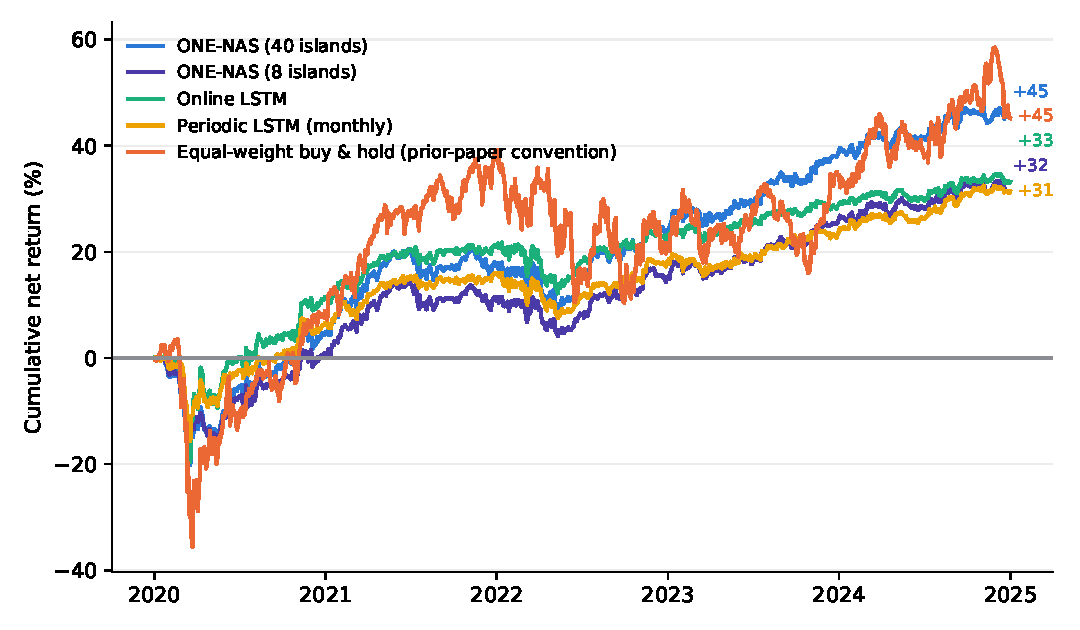
\includegraphics[width=0.92\textwidth]{net_curves.pdf}
\caption{Cumulative net return, 2022--2024 (books restarted at window
start). Buy-and-hold follows the prior-study benchmark convention.}
\label{fig:curves}
\end{figure*}

\begin{table}[t]
\centering
\footnotesize
\begin{tabular}{@{}lrr@{}}
\toprule
Comparison & $\Delta$net & paired $t$ \\
\midrule
vs.\ ONE-NAS (60 isl.)       & $-2.5$  & $-1.63$ \\
vs.\ ONE-NAS (20 isl.)       & $+0.2$  & $0.10$ \\
vs.\ Online LSTM             & $+16.2$ & $7.32$ \\
vs.\ Online GRU              & $+15.8$ & $6.59$ \\
vs.\ Periodic LSTM (monthly) & $+12.7$ & $6.66$ \\
vs.\ Online AR$^{a}$         & $+34.9$ & $2.22$ \\
\bottomrule
\end{tabular}
\par\smallskip
{\footnotesize
Comparisons are over all 40 (panel, seed) cells unless noted. Buy \& hold
trades once and is not seed-paired, so no paired test is reported against
it. $^{a}$Deterministic; one run per panel, so $n{=}4$.\par}
\caption{Paired significance for Table~\ref{tab:window}: within-cell
difference in net return (\%) between ONE-NAS (40 islands, sleeves book)
and each other arm, over the (panel, seed) cells the two arms share,
2022--2024.}
\label{tab:paired}
\end{table}

\begin{table}[t]
\centering
\footnotesize
\begin{tabular}{@{}l@{\hspace{3pt}}r@{\hspace{3pt}}r@{\hspace{3pt}}r@{\hspace{3pt}}r@{\hspace{3pt}}r@{}}
\toprule
Arm & $1\times$ & $2\times$ & $3\times$ & $5\times$ & B/E$^{a}$ \\
\midrule
ONE-NAS (60 isl.)   & $+30.1$ & $+27.2$ & $+24.4$ & $+18.8$ & $11.6\times$ \\
ONE-NAS (40 isl.)   & $+27.5$ & $+24.7$ & $+21.8$ & $+16.0$ & $10.6\times$ \\
ONE-NAS (20 isl.)   & $+27.4$ & $+24.4$ & $+21.5$ & $+15.6$ & $10.3\times$ \\
Periodic LSTM       & $+14.8$ & $+11.4$ & $+8.0$  & $+1.2$  & $5.4\times$ \\
Online GRU          & $+11.7$ & $+8.3$  & $+4.9$  & $-1.8$  & $4.5\times$ \\
Online LSTM         & $+11.3$ & $+8.1$  & $+4.9$  & $-1.5$  & $4.5\times$ \\
Online AR           & $-3.3$  & $-6.0$  & $-8.8$  & $-14.2$ & --- \\
\bottomrule
\end{tabular}
\par\smallskip
{\footnotesize
Scaling multiplies the realised per-name cost, so the cross-sectional
shape of costs is preserved and wide-spread names remain the expensive
ones. The $1\times$ column is the sleeves-book column of
Table~\ref{tab:window}. $^{a}$Break-even: the cost multiple at which net
return reaches zero.\par}
\caption{Cost sensitivity: net return (\%) on 2022--2024 as the realised
per-name transaction cost is scaled by the stated multiple. ONE-NAS
tolerates the harshest cost assumption of any arm.}
\label{tab:costs}
\end{table}

\begin{table*}[t]
\centering
\small
\begin{tabular}{@{}llrrrr@{}}
\toprule
Fleet & Window & Single & Ensemble & $\Delta$net ($t$) & $\Delta$Sharpe ($t$) \\
\midrule
60 isl.\ ($n{=}10$) & 2022--24 & $+1.0$ / $0.09$  & $+30.1$ / $0.93$ & $+29.1$ $(18.3)$ & $+0.84$ $(14.1)$ \\
60 isl.\ ($n{=}10$) & 2020--24 & $-2.1$ / $-0.01$ & $+49.8$ / $0.73$ & $+51.9$ $(16.7)$ & $+0.74$ $(14.3)$ \\
40 isl.\ ($n{=}10$) & 2022--24 & $+4.5$ / $0.21$  & $+27.5$ / $0.87$ & $+23.0$ $(18.2)$ & $+0.66$ $(14.7)$ \\
40 isl.\ ($n{=}10$) & 2020--24 & $+2.7$ / $0.08$  & $+45.6$ / $0.68$ & $+42.9$ $(14.6)$ & $+0.60$ $(13.4)$ \\
20 isl.\ ($n{=}10$) & 2022--24 & $+4.7$ / $0.25$  & $+27.4$ / $0.87$ & $+22.6$ $(14.9)$ & $+0.62$ $(14.9)$ \\
20 isl.\ ($n{=}10$) & 2020--24 & $-1.5$ / $0.02$  & $+41.6$ / $0.64$ & $+43.0$ $(14.8)$ & $+0.62$ $(16.7)$ \\
\midrule
40 isl.\ ($n{=}5$)$^{a}$ & 2016--19 & $+8.9$ / $0.30$  & $+36.7$ / $1.22$ & $+27.8$ $(7.5)$  & $+0.92$ $(6.6)$ \\
\bottomrule
\end{tabular}
\par\smallskip
{\footnotesize $^{a}$Replication on the 2016--2019 tuning-span fleets.\par}
\caption{Prediction rule, within-run paired: single global-best genome
vs.\ island-champion rank-mean ensemble from the same runs (sleeves book).
Net \% / Sharpe; $\Delta$ = ensemble $-$ single, paired $t$ over seeds.}
\label{tab:m1}
\end{table*}

\begin{figure}[t]
\centering
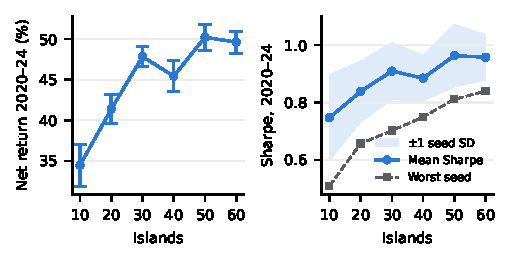
\includegraphics[width=\columnwidth]{islands_scaling.pdf}
\caption{Performance vs.\ island count (2020--2024, registered sleeves
book; 10 seeds $\times$ 4 panels at every width). Left: pooled net return
(mean $\pm$ SE). Right: Sharpe --- mean with $\pm$1 seed-SD band, and the
worst seed. Return and Sharpe climb steeply to about 30 islands and then
sit on a plateau ($+45$ to $+50$ net, Sharpe $0.88$--$0.96$) whose widths
are not separable at this replication; the worst seed improves
monotonically across the whole range ($0.51 \to 0.84$) while the seed SD
falls ($0.149 \to 0.079$), so width keeps buying reliability after it
stops buying mean return. The 40-island setting was fixed on the
2016--2019 tuning span before this curve was measured; the nominally
higher 50- and 60-island cells are eval-span measurements and are not
adopted.}
\label{fig:islands}
\end{figure}

\begin{table}[t]
\centering
\footnotesize
\begin{tabular}{@{}l@{\hspace{4pt}}r@{\hspace{4pt}}r@{\hspace{4pt}}r@{\hspace{4pt}}r@{}}
\toprule
Arm & bps/day & \%/yr & NW $t$ & Beta \\
\midrule
ONE-NAS (60 islands)     & $+3.47$ & $+8.7$ & $+2.32$ & $+0.124$ \\
ONE-NAS (40 islands)     & $+3.15$ & $+7.9$ & $+2.14$ & $+0.120$ \\
ONE-NAS (20 islands)     & $+2.87$ & $+7.2$ & $+2.04$ & $+0.108$ \\
Periodic LSTM (monthly)  & $+2.27$ & $+5.7$ & $+1.89$ & $+0.083$ \\
Online LSTM              & $+2.24$ & $+5.6$ & $+1.73$ & $+0.131$ \\
Online GRU               & $+1.54$ & $+3.9$ & $+1.42$ & $+0.106$ \\
Online AR                & $-1.35$ & $-3.4$ & $-1.05$ & $+0.007$ \\
\bottomrule
\end{tabular}
\caption{Factor-adjusted alphas: pooled daily book returns regressed on
the Fama--French three factors plus momentum, 2020--2024, Newey--West lag
10.}
\label{tab:alphas}
\end{table}

\begin{table}[t]
\centering
\footnotesize
\begin{tabular}{@{}l@{\hspace{3pt}}c@{\hspace{3pt}}c@{\hspace{3pt}}c@{\hspace{3pt}}c@{\hspace{3pt}}c@{}}
\toprule
Fleet & $N$ & $\rho$ & Member & Ensemble & Predicted \\
\midrule
20 isl., 2020--24 & 20 & 0.180 & $+0.0056$ & $+0.0117$ & $+0.0120$ \\
40 isl., 2020--24 & 40 & 0.172 & $+0.0058$ & $+0.0128$ & $+0.0132$ \\
60 isl., 2020--24 & 60 & 0.177 & $+0.0060$ & $+0.0131$ & $+0.0137$ \\
\midrule
40 isl., 2016--19 & 40 & 0.187 & $+0.0078$ & $+0.0166$ & $+0.0171$ \\
\bottomrule
\end{tabular}
\caption{Ensemble diversity mechanism: member rank IC, pairwise member
prediction correlation $\rho$, measured ensemble IC, and the
equicorrelated averaging prediction $m\sqrt{N/(1+(N-1)\rho)}$.}
\label{tab:diversity}
\end{table}

\begin{table}[t]
\centering
\small
\begin{tabular}{@{}lr@{\quad}lr@{}}
\toprule
Configuration & $\Delta$net & Configuration & $\Delta$net \\
\midrule
C0 (registered)      & $+3.9$  & NTS 600            & $+12.8$ \\
Select: IC-gated     & $+0.5$  & Rounds 2           & $+11.0$ \\
Select: IC           & $+2.8$  & PER $\alpha$ 0.4   & $+4.0$  \\
Target: 5-day CS     & $+4.5$  & PER $\alpha$ 0.8   & $+11.7$ \\
5-day CS + IC-gated  & $+1.8$  & PER $\lambda{\times}3$ & $+20.6$ \\
Elite 5 / gen 10     & $+9.6$  & BP epochs 20       & $+12.5$ \\
Elite 5 / gen 15     & $+11.1$ & Repop.\ 25         & $+7.0$  \\
Repop.\ 100          & $+9.6$  & PER off (uniform)  & $+9.3$  \\
\bottomrule
\end{tabular}
\par\smallskip
{\footnotesize Mean $+8.3$; $n{=}6$ runs per cell (2 panels $\times$ 3
seeds).\par}
\caption{Ensembling gain (ensemble $-$ single champion, within-run, net \%
on 2016--2019) inside every trained hyperparameter configuration; positive
in 16/16 cells.}
\label{tab:invariance}
\end{table}

\begin{table}[t]
\centering
\small
\begin{tabular}{@{}lr@{}}
\toprule
Population evolving online since 2020-01 & $+26.5$ \\
Cold start at 2022-01                     & $+12.3$ \\
\bottomrule
\end{tabular}
\caption{Online continuity: pooled net (\%) on 2022--2024, frozen 8-island
configuration.}
\label{tab:continuity}
\end{table}

\begin{table}[t]
\centering
\footnotesize
\begin{tabular}{@{}l@{\hspace{4pt}}l@{}}
\toprule
Hyperparameter & Value \\
\midrule
Islands & 40 (headline); 8 (reg.) \\
Elite population / island & 8 \\
Generated / island / generation & 5 \\
Repopulation frequency & every 50 gen. \\
Selection metric & validation MSE \\
Prediction rule & champion rank-mean \\
Target & 1-day CS rank-normal \\
Seq.\ len.\ / step / val.\ sets & 40 / 5 / 5 \\
Train subseq.\ / genome & 2000 \\
Backprop.\ epochs / genome & 10 \\
Replay (PER) $\alpha$, $\lambda$, $\epsilon$ & 0.6, 0.007, $10^{-8}$ \\
Rounds / generation & 1 \\
Node types & simple, UGRNN, MGU, \\
 & GRU, $\Delta$-RNN, LSTM \\
Mut.\ / intra- / inter-crossover & 0.7 / 0.2 / 0.1 \\
Warm-up generations & 50 \\
\bottomrule
\end{tabular}
\caption{ONE-NAS hyperparameter settings (selected on 2016--2019
validation data, disjoint from the evaluation span). Replay sampling
ablated: PER vs.\ uniform shows no advantage on the tuning objective
($\Delta$IC $-0.0024$, $t{=}-1.9$).}
\label{tab:hps}
\end{table}
